\documentclass{article}
\title{test}
\author{test2}
\date{\today}
\usepackage[colorlinks=true,allcolors=green]{hyperref}
\usepackage{fullpage, amsmath,polski}
\usepackage{graphicx}
\begin{document}\huge
\begin{figure}
        \centering
        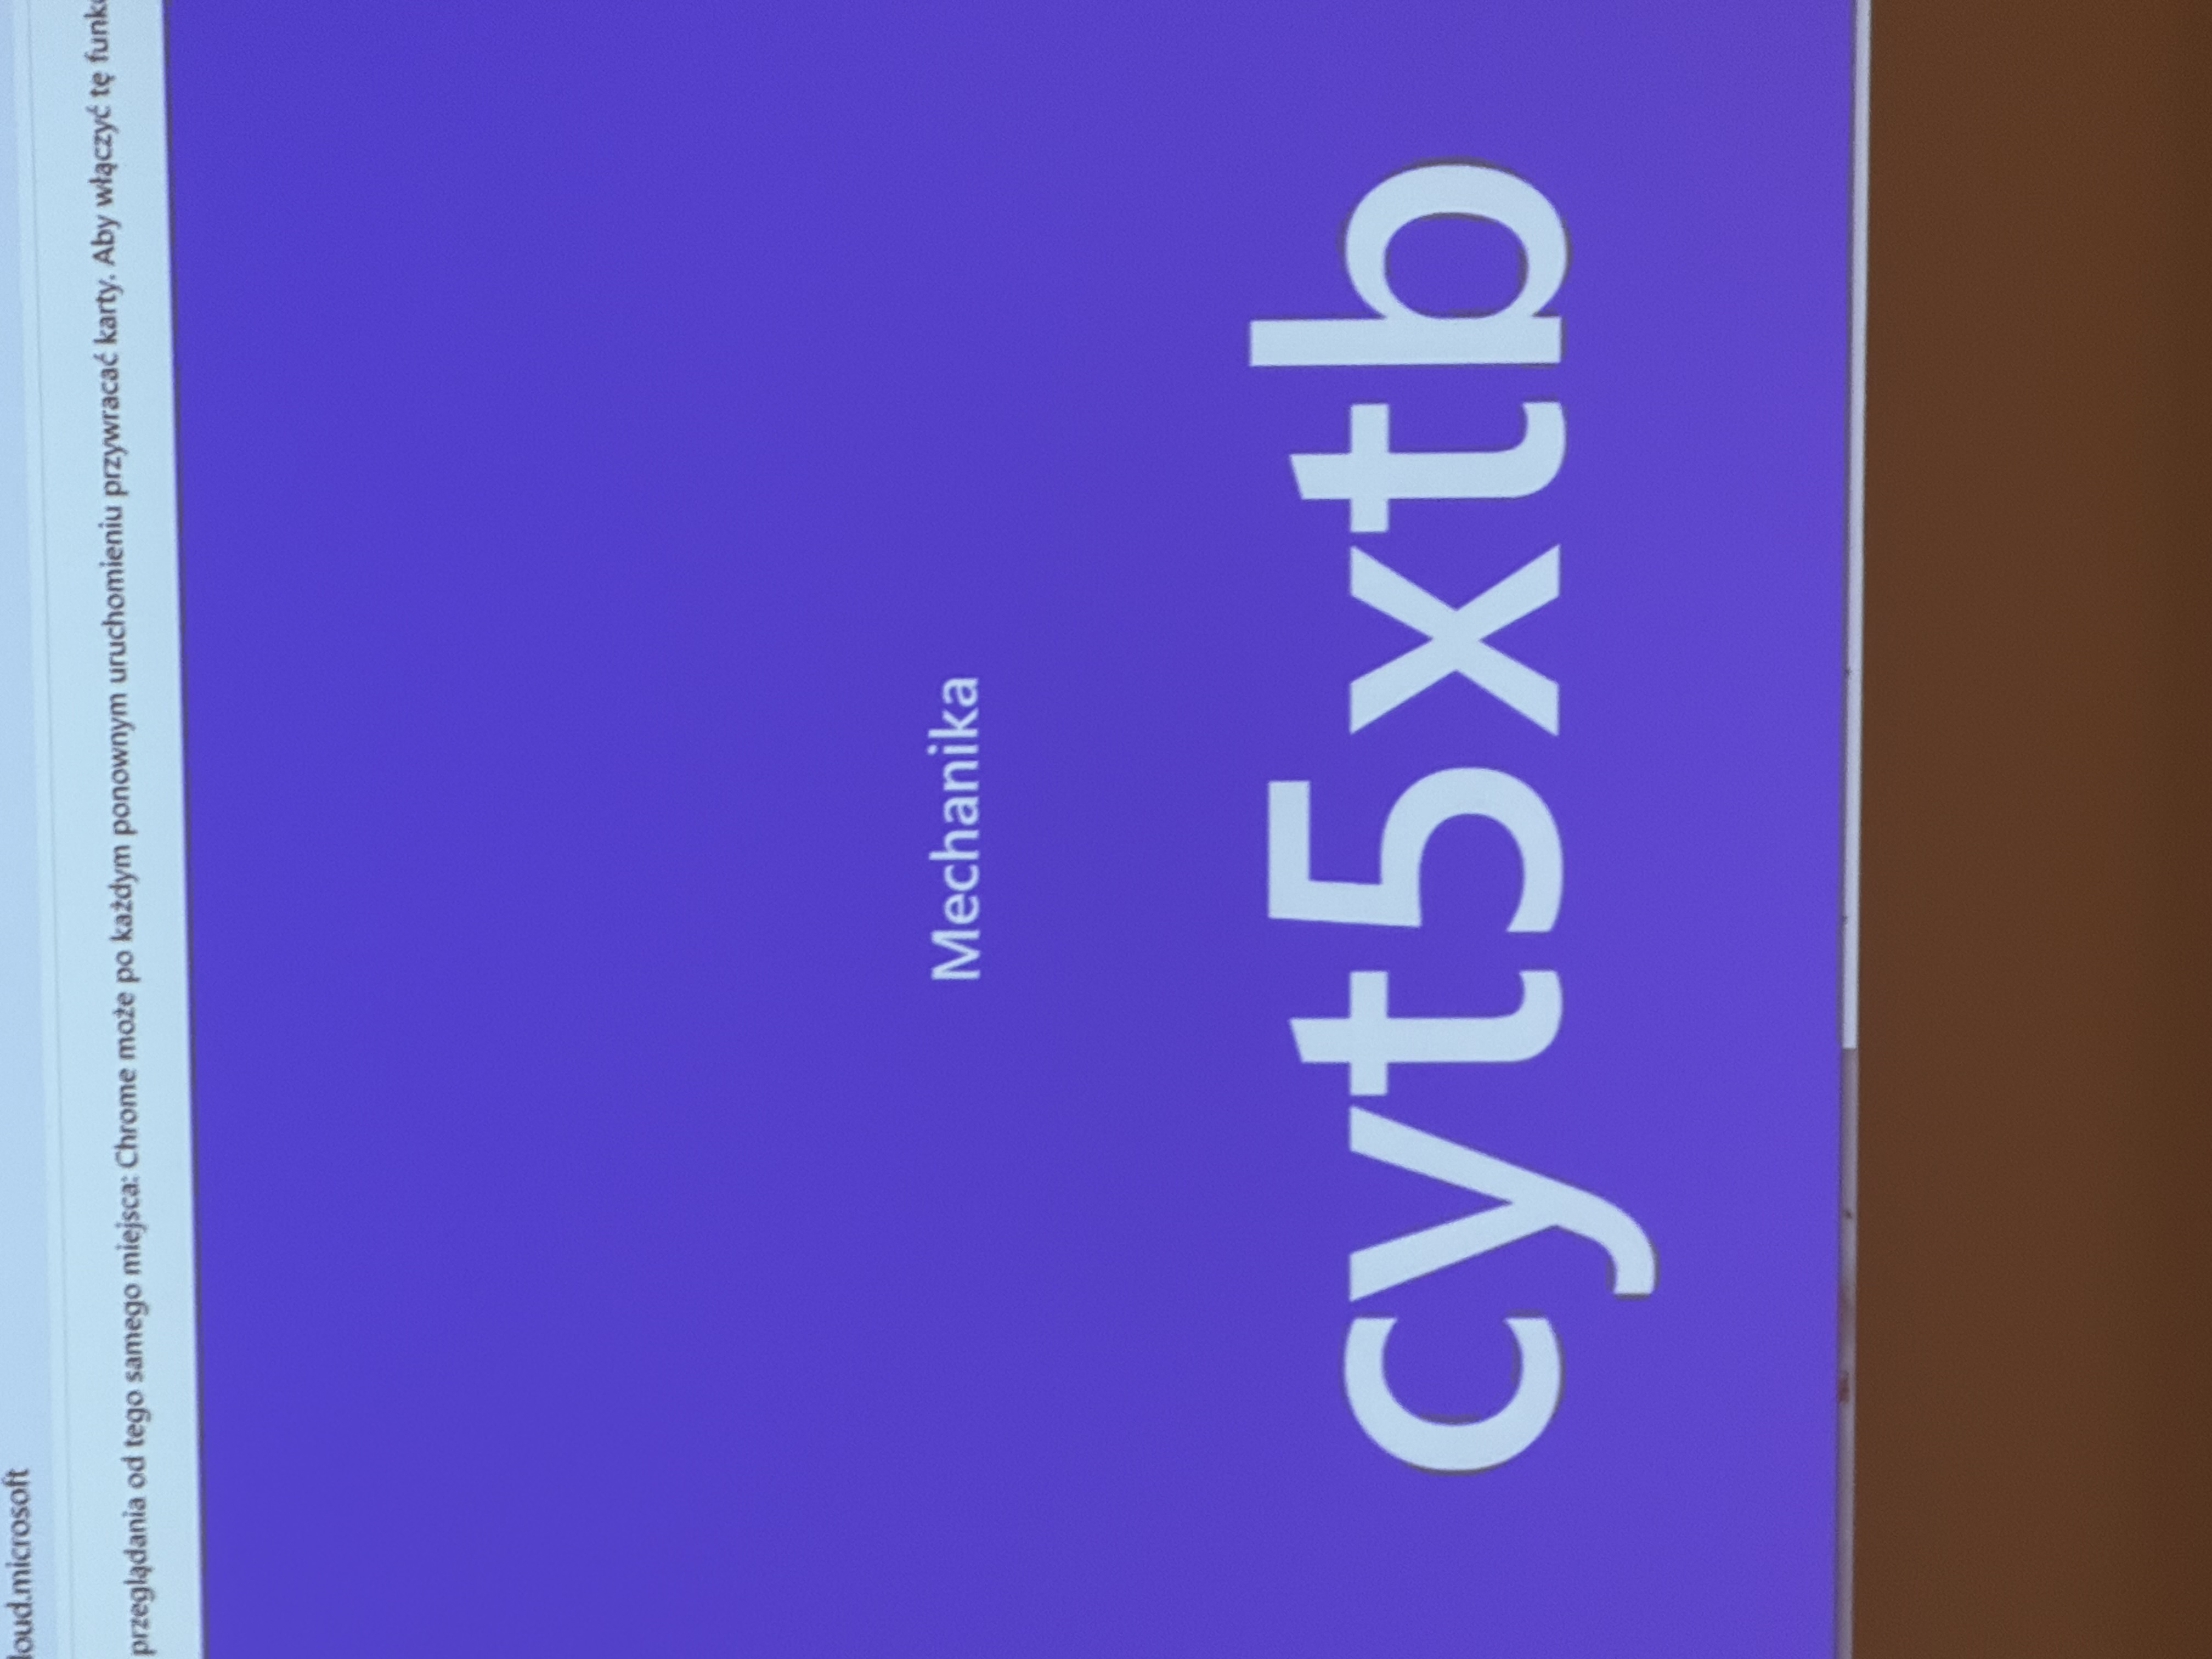
\includegraphics[width=30px]{IMG_2728.jpeg}
        \caption{Enter Caption}
        \label{fig:placeholder}
    \end{figure}
        \maketitle
    Akademia G-H\footnote{\href{https://www.agh.edu.pl/o-agh/historia-i-tradycja}{zał. 1913}}
    \begin{equation}\label{Euler}
e^{i\pi}=-1
    \end{equation}
    \eqref{Euler} na stronie \pageref{Euler}
\end{document}